\documentclass{beamer}
\usetheme{}
\usecolortheme{dolphin}           
\useinnertheme{circles}
\setbeamertemplate{itemize items}[default]
\setbeamertemplate{enumerate items}[default]
\usepackage[T1]{fontenc}
\usepackage[utf8]{inputenc}
\usepackage{lmodern}
\usepackage{amsmath}
\usepackage{booktabs} 
\usepackage{graphicx}        
\usepackage{array}
\usepackage{color}
\makeatletter
\def\zapcolorreset{\let\reset@color\relax\ignorespaces}
\def\colorrows#1{\noalign{\aftergroup\zapcolorreset#1}\ignorespaces}
\makeatother
\setbeamertemplate{navigation symbols}{}
\setbeamertemplate{footline}[frame number]

%--------------------------------------
\title{Macroeconomic integration}
\author{School of Economics, University College Dublin}
\date{Spring 2018}
\begin{document}

%--------------------------------------
\begin{frame}
 \titlepage
\end{frame}
%--------------------------------------

%--------------------------------------
\begin{frame}
  \textbf{Balassa's six stages of macroeconomic integration}
  \begin{enumerate}
    \item Preferential customs area
    \item Free trade area
    \item Customs union
    \item Common market
    \item Economic and monetary union
    \item Political union
  \end{enumerate}
\end{frame}
%--------------------------------------

%--------------------------------------
\begin{frame}
  \textbf{EU} currently at stage 4
  \begin{itemize}
    \item All member countries part of the common market
    \item Some member of a monetary union (eurozone)
  \end{itemize}
  \medskip
 \textbf{Eurozone} member states at stage 5\\
  \medskip
  Members of the eurozone can set \textbf{fiscal} policy but not \textbf{monetary} policy
  \begin{itemize}
    \item Autonomy over public spending and taxing
    \item Can't set interest rates or depreciate/appreciate currency
  \end{itemize}
\end{frame}
%--------------------------------------

%--------------------------------------
\begin{frame}
  \textbf{European debt crisis} illustrated limitations of integration
  \begin{itemize}
    \item Due to heterogeneity across member states
  \end{itemize}
  \medskip
  For future integration two options (besides status quo)
  \begin{enumerate}
    \item Abolish euro: move back to stage 4
    \item Further integration: moving towards stage 6
    \begin{enumerate}[i]
      \item Banking union (2014)
      \item Fiscal union
      \item Political union
    \end{enumerate}    
  \end{enumerate}  
\end{frame}
%--------------------------------------

%--------------------------------------
\begin{frame}
  \textbf{Briefly:} the EU's Banking Union
  \begin{itemize}
    \item Supervision of EU banks
    \item Response to EU financial crisis; deeper financial integration eurozone banking system    
  \end{itemize}
  \medskip
  Mainly guidelines on 
  \begin{enumerate}[i]
    \item Prudential requirements for banks
    \item Depositor protection
    \item Managing failing banks
  \end{enumerate}
  \medskip
  Two pillars in place
  \begin{enumerate}
    \item Single Supervisory Mechanism (SSM)
    \item Single Resolution Mechanism (SRM)
  \end{enumerate}
  Lacking: European deposit insurance scheme
\end{frame}
%--------------------------------------


%--------------------------------------
\begin{frame}
  \textbf{Political project}\\
  Two schools of thought on integration\footnote{Spoloare (2014), 'What is European integration really about? A political guide for economists', Journal of Economic Perspectives.}
  \begin{enumerate}
    \item Intergovernmentalism
    \begin{itemize}
      \item National governments are in charge
      \item States can use EU for their own goals
    \end{itemize}
    \medskip
    \item Functionalism
    \begin{itemize}
      \item Integration pushed by elites and interest groups that transcend national boundaries
      \item Dynamic effect of transferring functions from national government to Brussels
    \end{itemize}
  \end{enumerate}
\end{frame}
%--------------------------------------

%--------------------------------------
\begin{frame}
  European integration therefore either
  \medskip
  \begin{enumerate}
    \item Follows from national economic interests
    \medskip
    \item Or is a path towards political integration
  \end{enumerate}  
\end{frame}
%--------------------------------------

%--------------------------------------
\begin{frame}
  Functionalism works through a \textbf{chain reaction}
  \begin{enumerate}
    \item Move functions in narrow areas from government to supranational body
    \item Over time will lead to more integration 
  \end{enumerate}
  \medskip
  Further centralisation will follow through +ve/-ve mechanisms
  \begin{itemize}
    \item +ve: through learning, changing preferences
    \item -ve: generating problems and crises
  \end{itemize}
\end{frame}
%--------------------------------------

%--------------------------------------
\begin{frame}
  Further centralisation through -ve mechanism implies that national politicians don't anticipate chain reaction  
  \medskip
  \begin{enumerate}
    \item Short horizons
    \item Asymmetric information
    \item Democratic deficit
  \end{enumerate}
\end{frame}
%--------------------------------------

%--------------------------------------
\begin{frame}
  \begin{figure}
    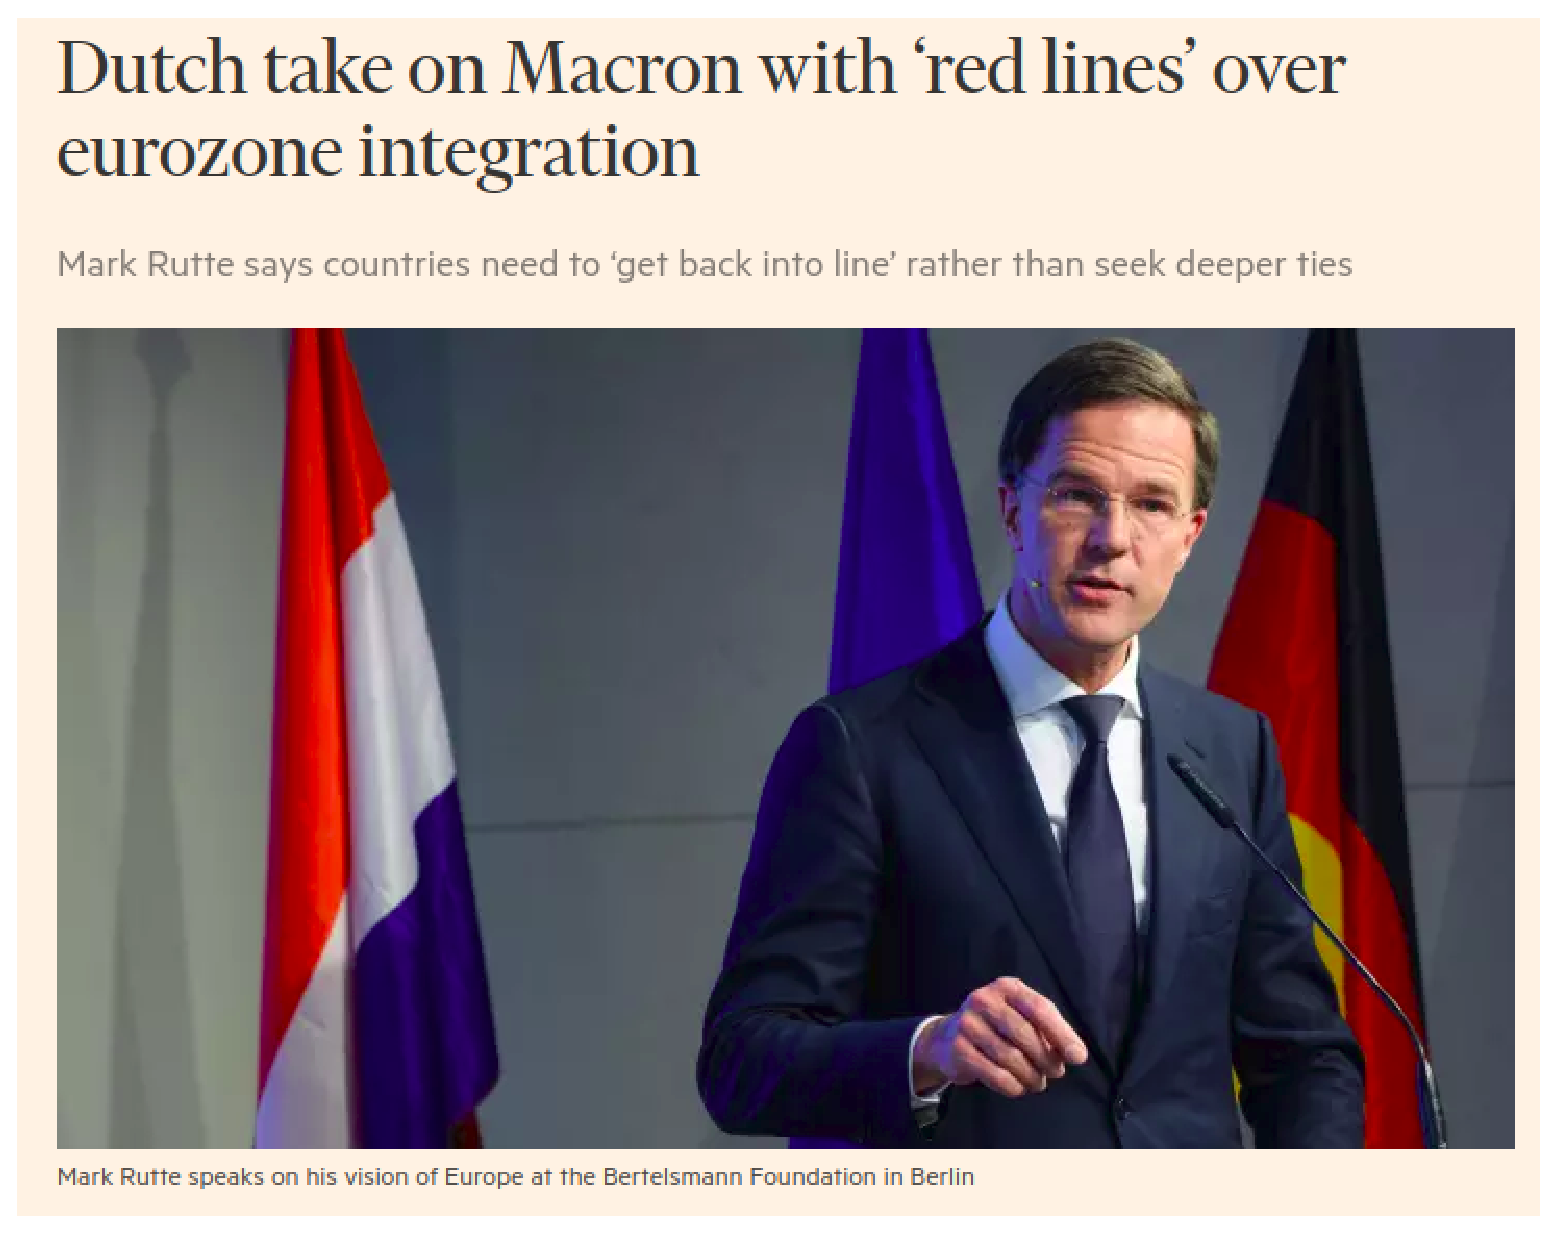
\includegraphics[scale=.4]{rutte.eps}
  \end{figure}
\end{frame}
%--------------------------------------

%--------------------------------------
\begin{frame}
  \textbf{Economic responsiblity}
  \begin{quote}
    It’s time to get back into line. The recipe for a larger cake is not centralised bailout funds and printing more money, but structural reforms and sound budgets
  \end{quote}
  \textbf{EU project as a whole}
  \begin{quote}
   the EU is not an unstoppable train speeding towards federalism
 \end{quote}
 \textbf{Role of European Commission in context of crisis} 
 \begin{quote}
   the commission should work more for EU governments and not the other way round
 \end{quote}
 \textbf{Concerning budget rules}
 \begin{quote}
   There must be no political assessment
 \end{quote}
\end{frame}
%--------------------------------------

%--------------------------------------
\begin{frame}
  Examining macroeconomics of European integration will focus on
  \begin{enumerate}
    \item Monetary policy
    \item Fiscal policy
    \item Economic growth
  \end{enumerate}
  \medskip
  Start with some basic economics
\end{frame}
%--------------------------------------

%--------------------------------------
\begin{frame}
  \begin{figure}
    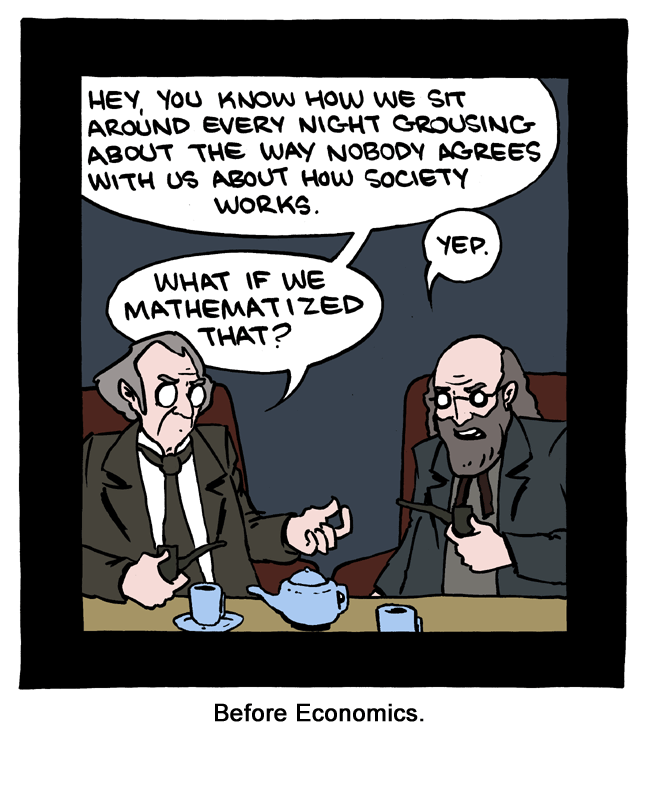
\includegraphics[scale=.6]{smbc.eps}
  \end{figure}
  Source: Saturday Morning Breakfast Comics
\end{frame}
%--------------------------------------

%--------------------------------------
\begin{frame}
  \textbf{Closed economy}
  \begin{align}
    Y=C+I+G
  \end{align}
  \medskip
  Equilibrium GDP given by
  \begin{align}
    Y=C(Y) + I +G
  \end{align}
  $C(Y)$
  \begin{enumerate}
    \item Consumers spend more when they earn more
    \item Consumers earn more when firms produce more
    \begin{enumerate}
      \item Firms invest borrowing at interest rate $i$: when $i$ increases, $I$ and $C$ decrease   
    \end{enumerate}
  \end{enumerate}
\end{frame}
%--------------------------------------

%--------------------------------------
\begin{frame}
  \begin{align*}
    Y=C(Y) + I + G
  \end{align*}
  \medskip
  Government can change spending $G$
  \begin{itemize}
    \item e.g. increase spending in infrastructure
  \end{itemize}
  \medskip
  $G$ set by fiscal policy; relevant in business cycle context
  \begin{itemize}
    \item Expansionary policy will increase $G$ \& reduce taxes
  \end{itemize}
\end{frame}
%--------------------------------------

%--------------------------------------
\begin{frame}
  \begin{figure}
    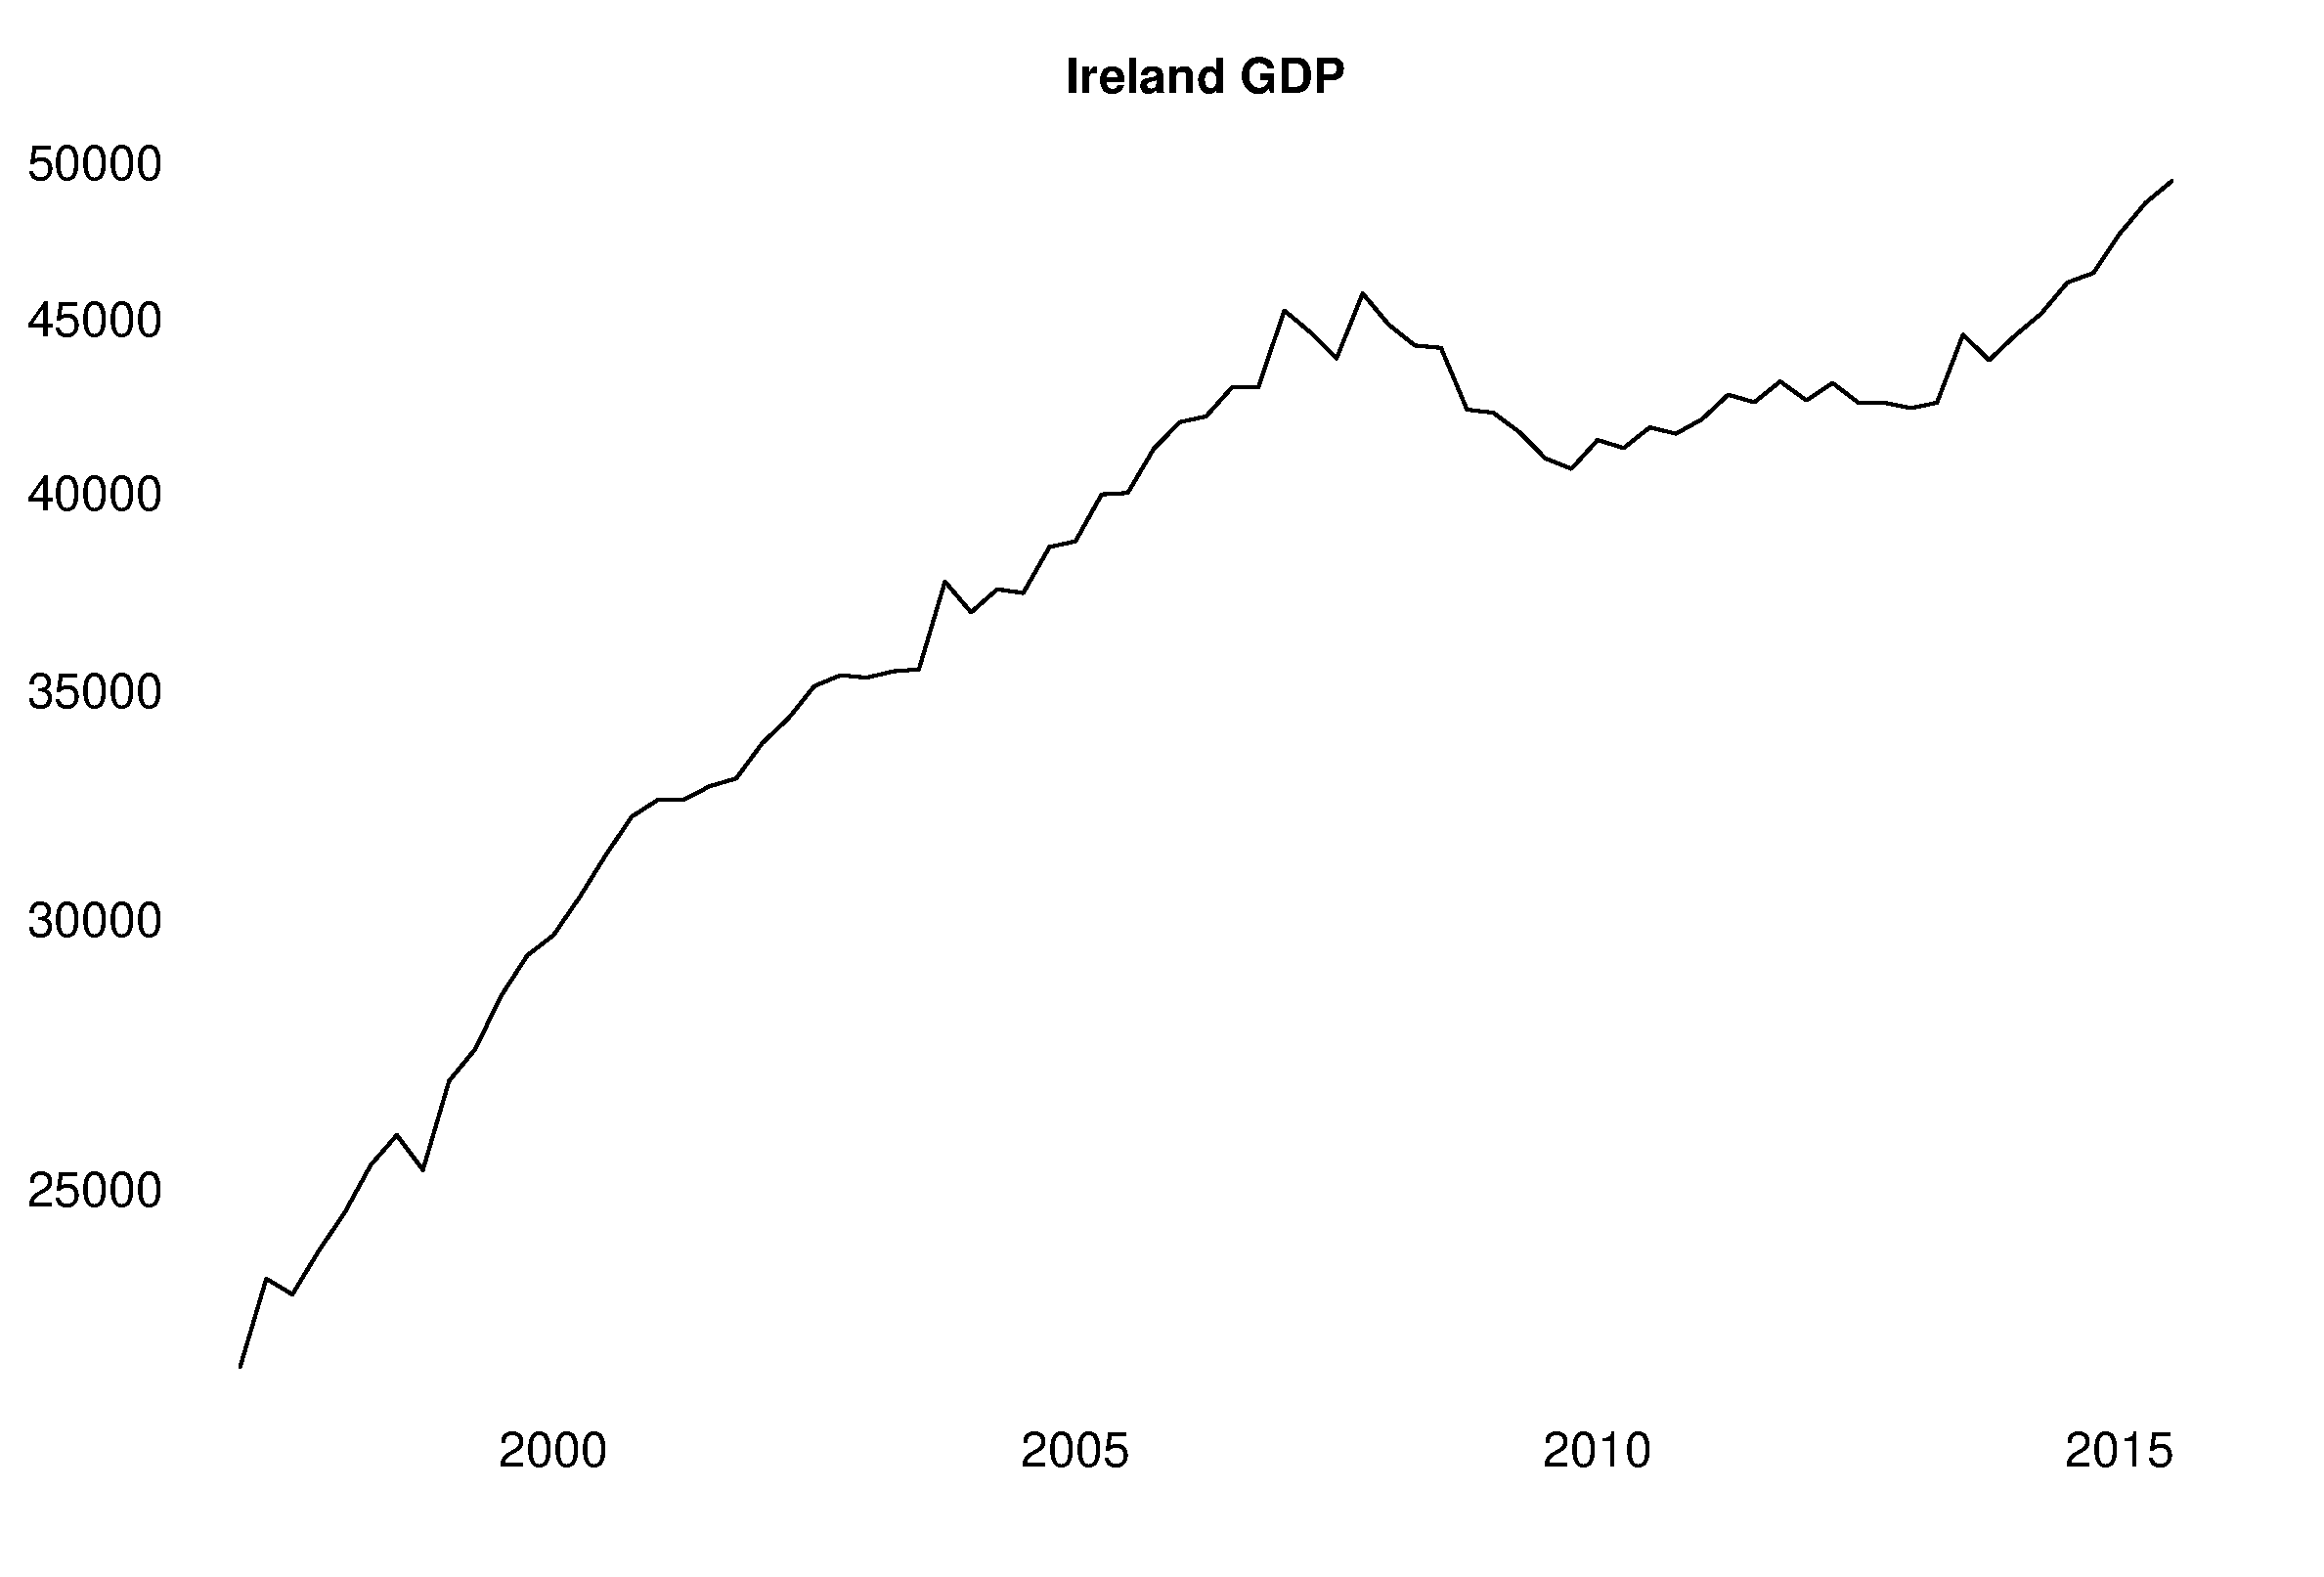
\includegraphics[scale=.25]{ire_gdp.eps}
  \end{figure}
\end{frame}
%--------------------------------------

%--------------------------------------
\begin{frame}
  \begin{figure}
    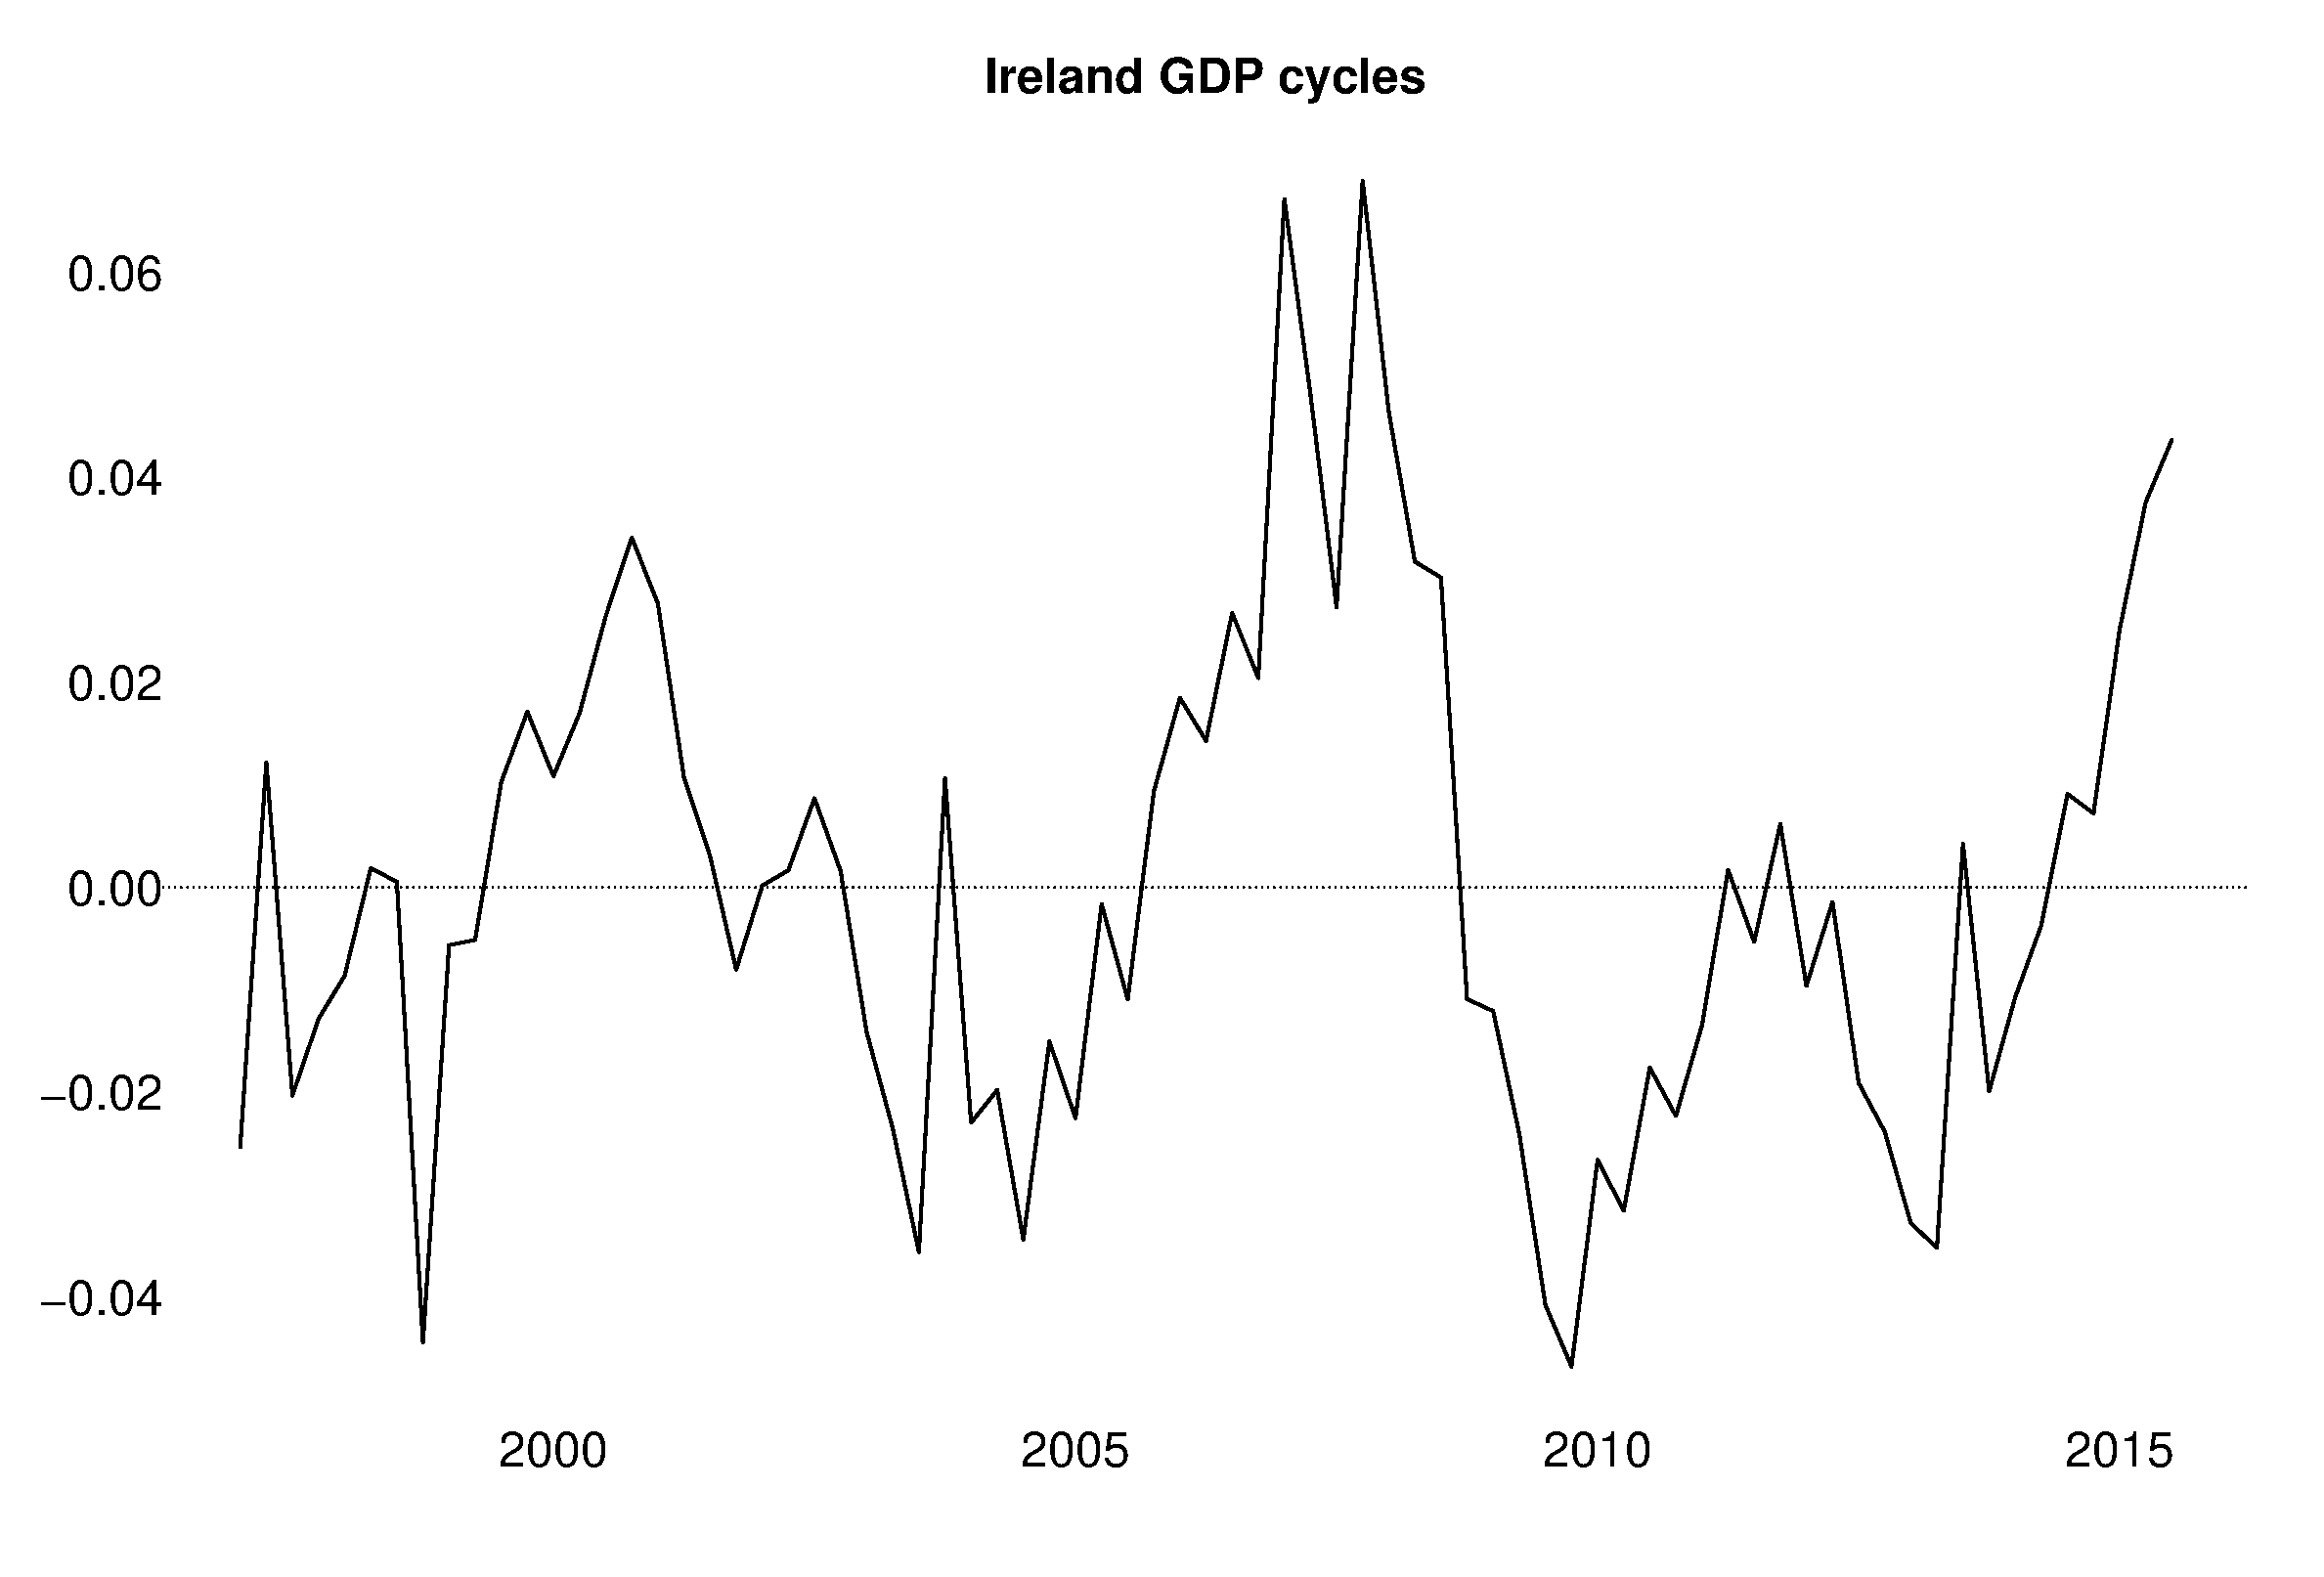
\includegraphics[scale=.25]{ire_gdp_hp.eps}
  \end{figure}
\end{frame}
%--------------------------------------

%--------------------------------------
\begin{frame}
  \begin{figure}
    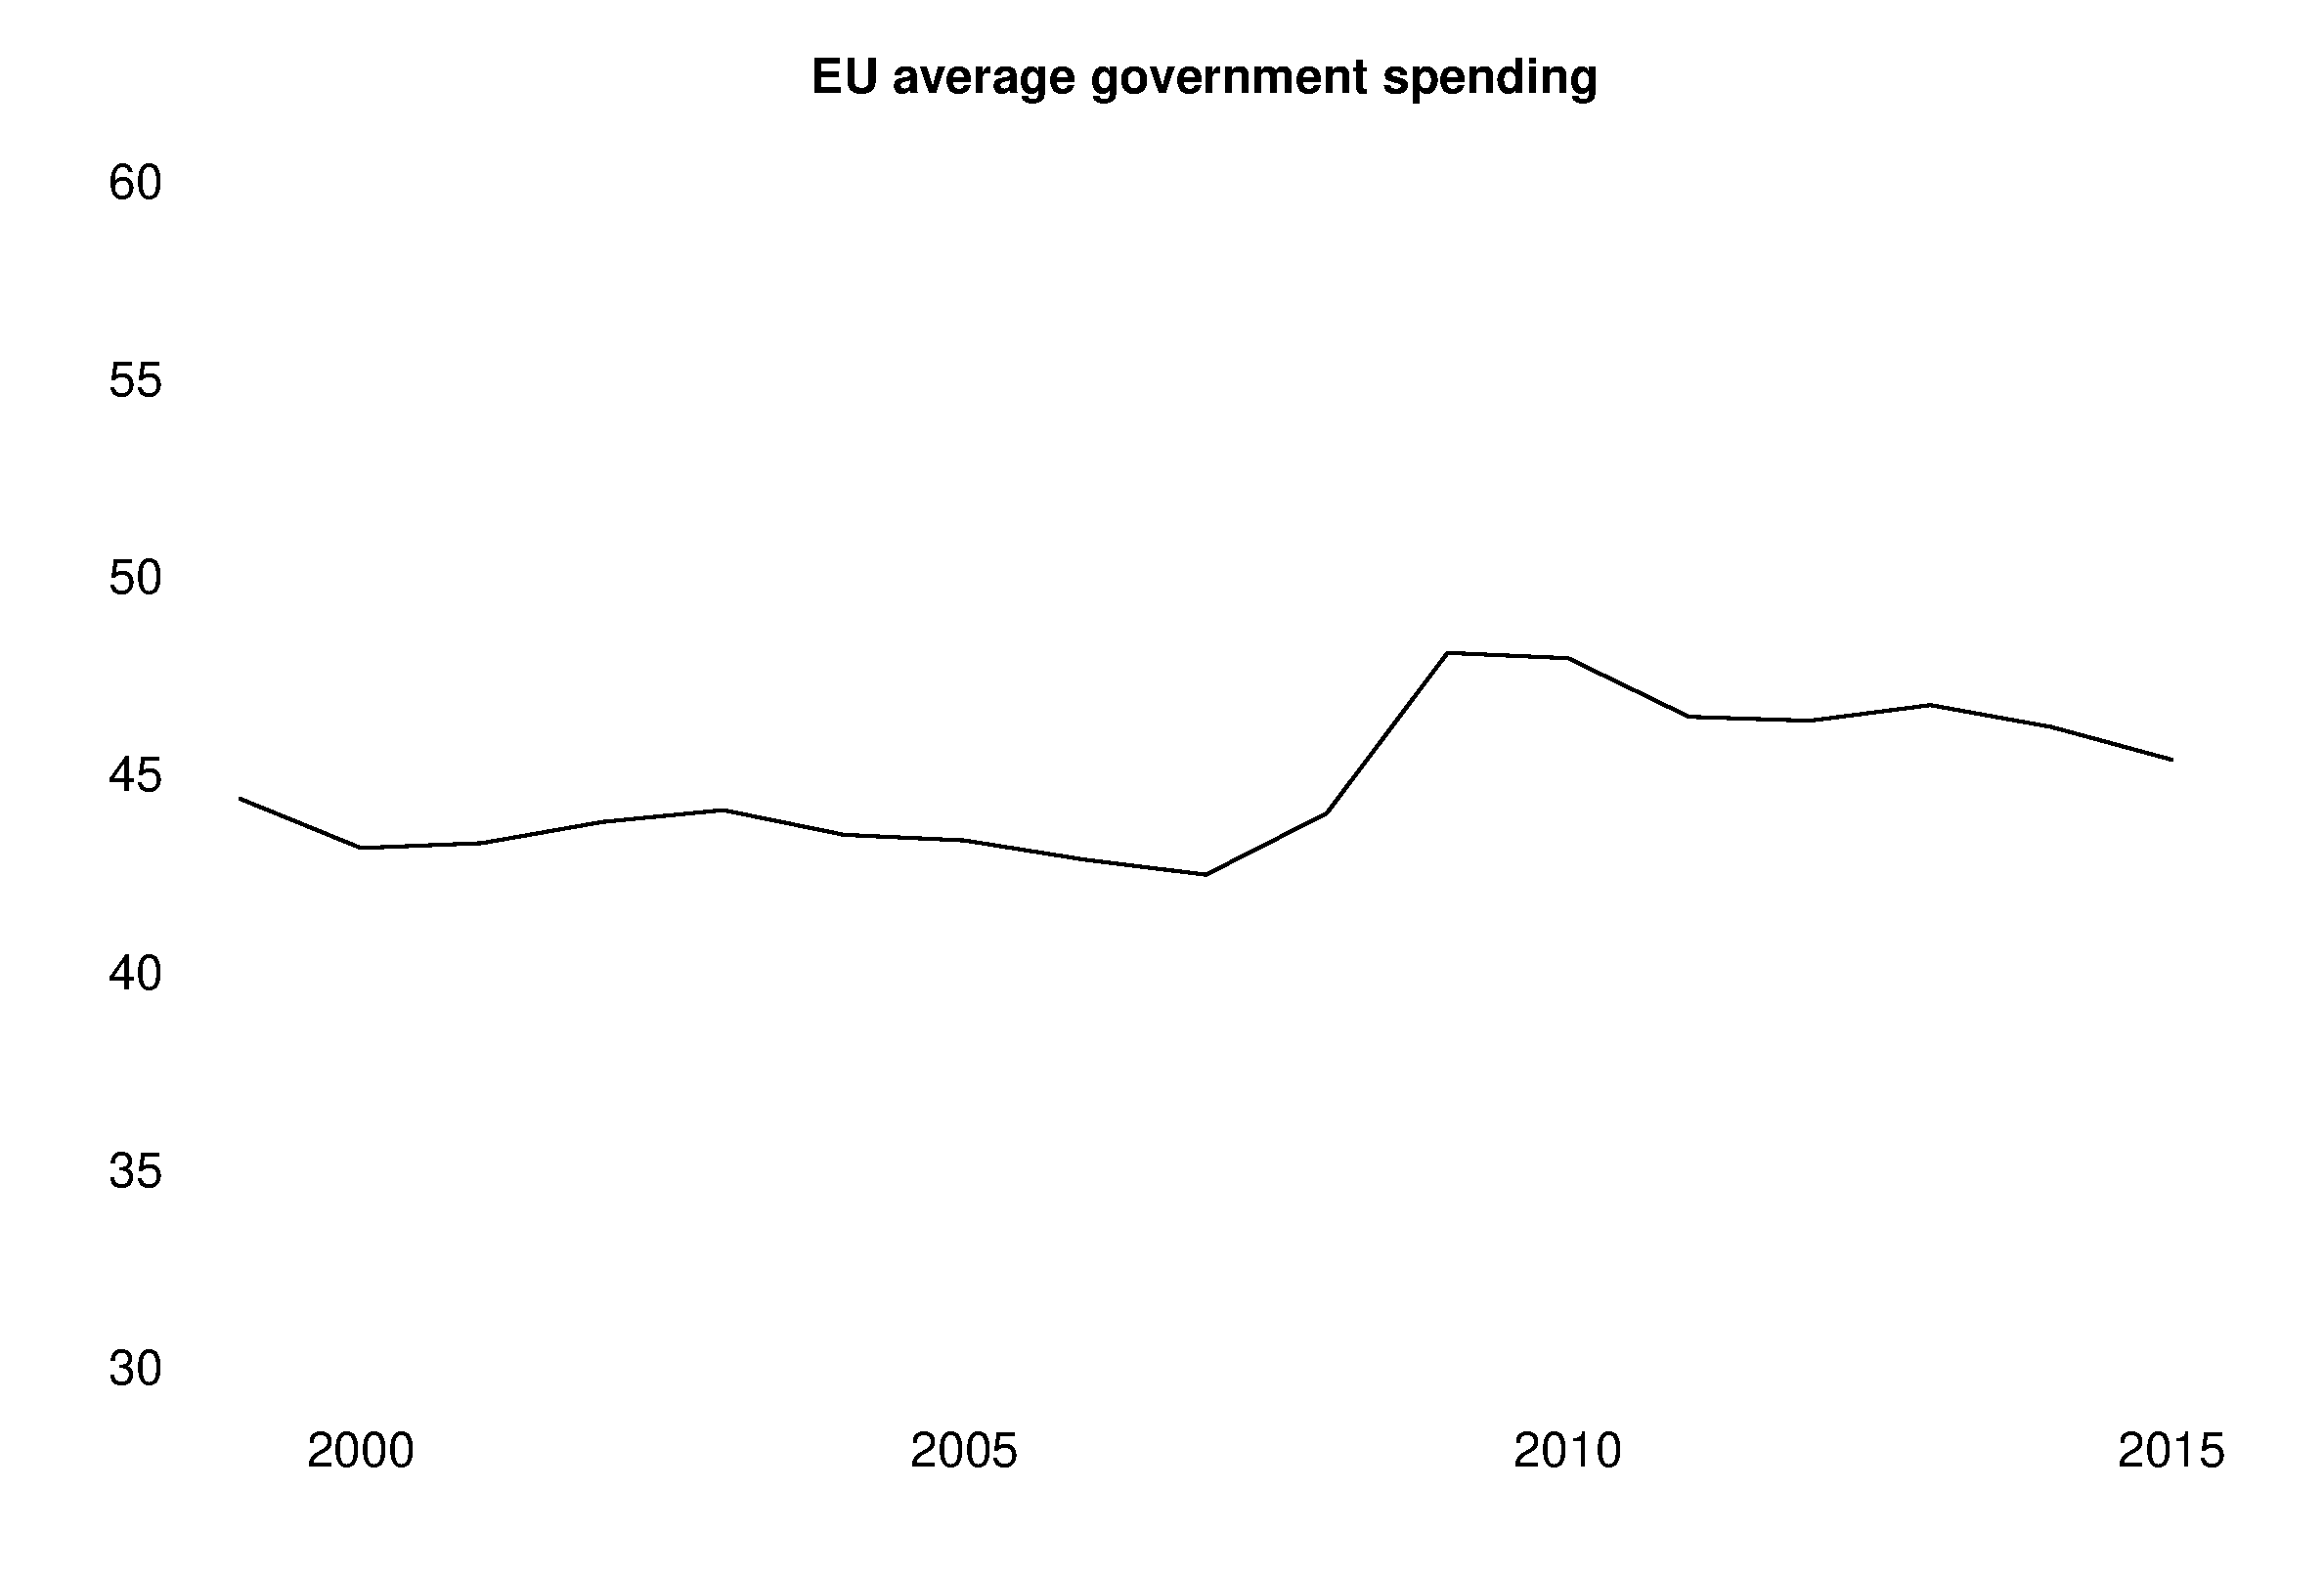
\includegraphics[scale=.25]{eu_G.eps}
  \end{figure}
\end{frame}
%--------------------------------------

%--------------------------------------
\begin{frame}
  Role of \textbf{financial markets}
  \begin{itemize}
     \item Collect savings from households/firms
     \item Lend money to households/firm and public authorities
   \end{itemize} 
   \medskip
   Number of feature of the financial market that are of interest
  \begin{enumerate}
    \item Most people rely on banks for savings deposits
    \item Finance is associated with risk
    \item Price associated with risk
    \item Financial intermediaries deal with each other, continuously    
  \end{enumerate}
\end{frame}
%--------------------------------------

%--------------------------------------
\begin{frame}
  Financial markets are subject to 
  \begin{enumerate}
    \item Regulations
    \item Monetary policy
  \end{enumerate}
  \medskip
  Monetary policy is set by central bank, which generally has two objectives
  \medskip
  \begin{enumerate}
    \item Control inflation
    \item Stabilise economy
  \end{enumerate}  
\end{frame}
%--------------------------------------

%--------------------------------------
\begin{frame}
  \textbf{Open economy}  
  \begin{align}
    Y=C+I+G+X-M
  \end{align}
  $X$ is exports\\
  $M$ is imports\\
  $X-M$ is current account.  
  \medskip
  \begin{itemize}
    \item Goods and services markets become interdependent across countries
  \end{itemize}
\end{frame}
%--------------------------------------

%--------------------------------------
\begin{frame}
  \textbf{Interest rate parity condition}
  \begin{align}
    1+i_t = (1+r^*) \frac{E^e_{t+1}}{E_t}
  \end{align}
  $i_t$, domestic interest rate\\
  $r^*$, foreign bond return\\
  $E^e_{t+1}$, expected exchange rate\\
  \begin{itemize}
    \item Higher interest rate when exchange rate is expected to depreciate: to prevent capital outflows
    \item Lower interest rate when exchange rate is expected to appreciate
  \end{itemize}
\end{frame}
%--------------------------------------

%--------------------------------------
\begin{frame}
  \begin{figure}
    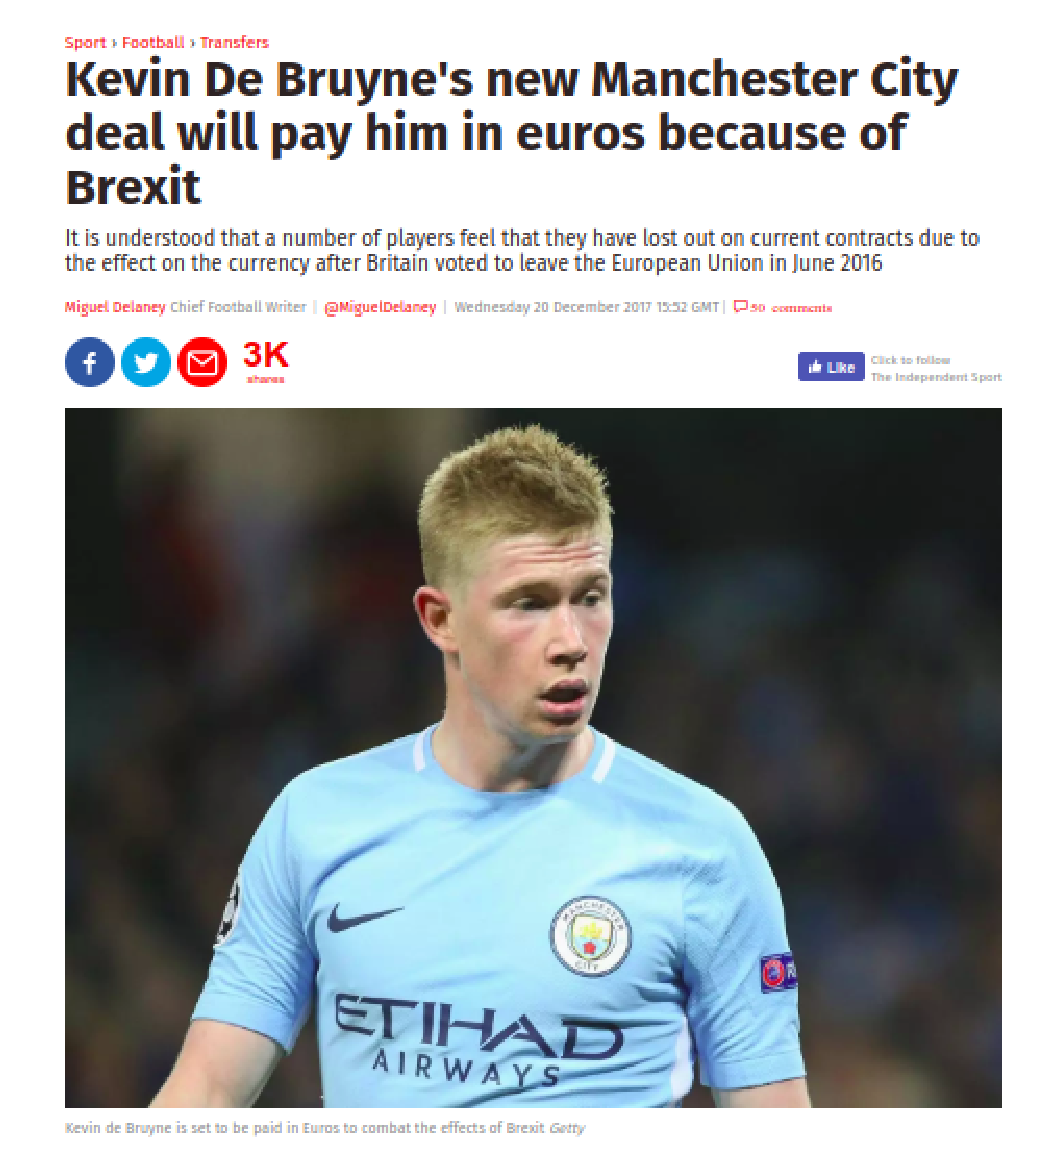
\includegraphics[scale=.5]{de_bruyne.eps}
  \end{figure}
\end{frame}
%--------------------------------------

%--------------------------------------
\begin{frame}
  Can restate parity condition as
  \begin{align}
    i_t = i^*_t +  \frac{E^e_{t+1}}{E_t}
  \end{align}
  \begin{quote}
    Domestic interest rate = Foreign interest rate + Expected exchange rate depreciation
  \end{quote}
\end{frame}
%--------------------------------------

%--------------------------------------
\begin{frame}
  \begin{figure}
    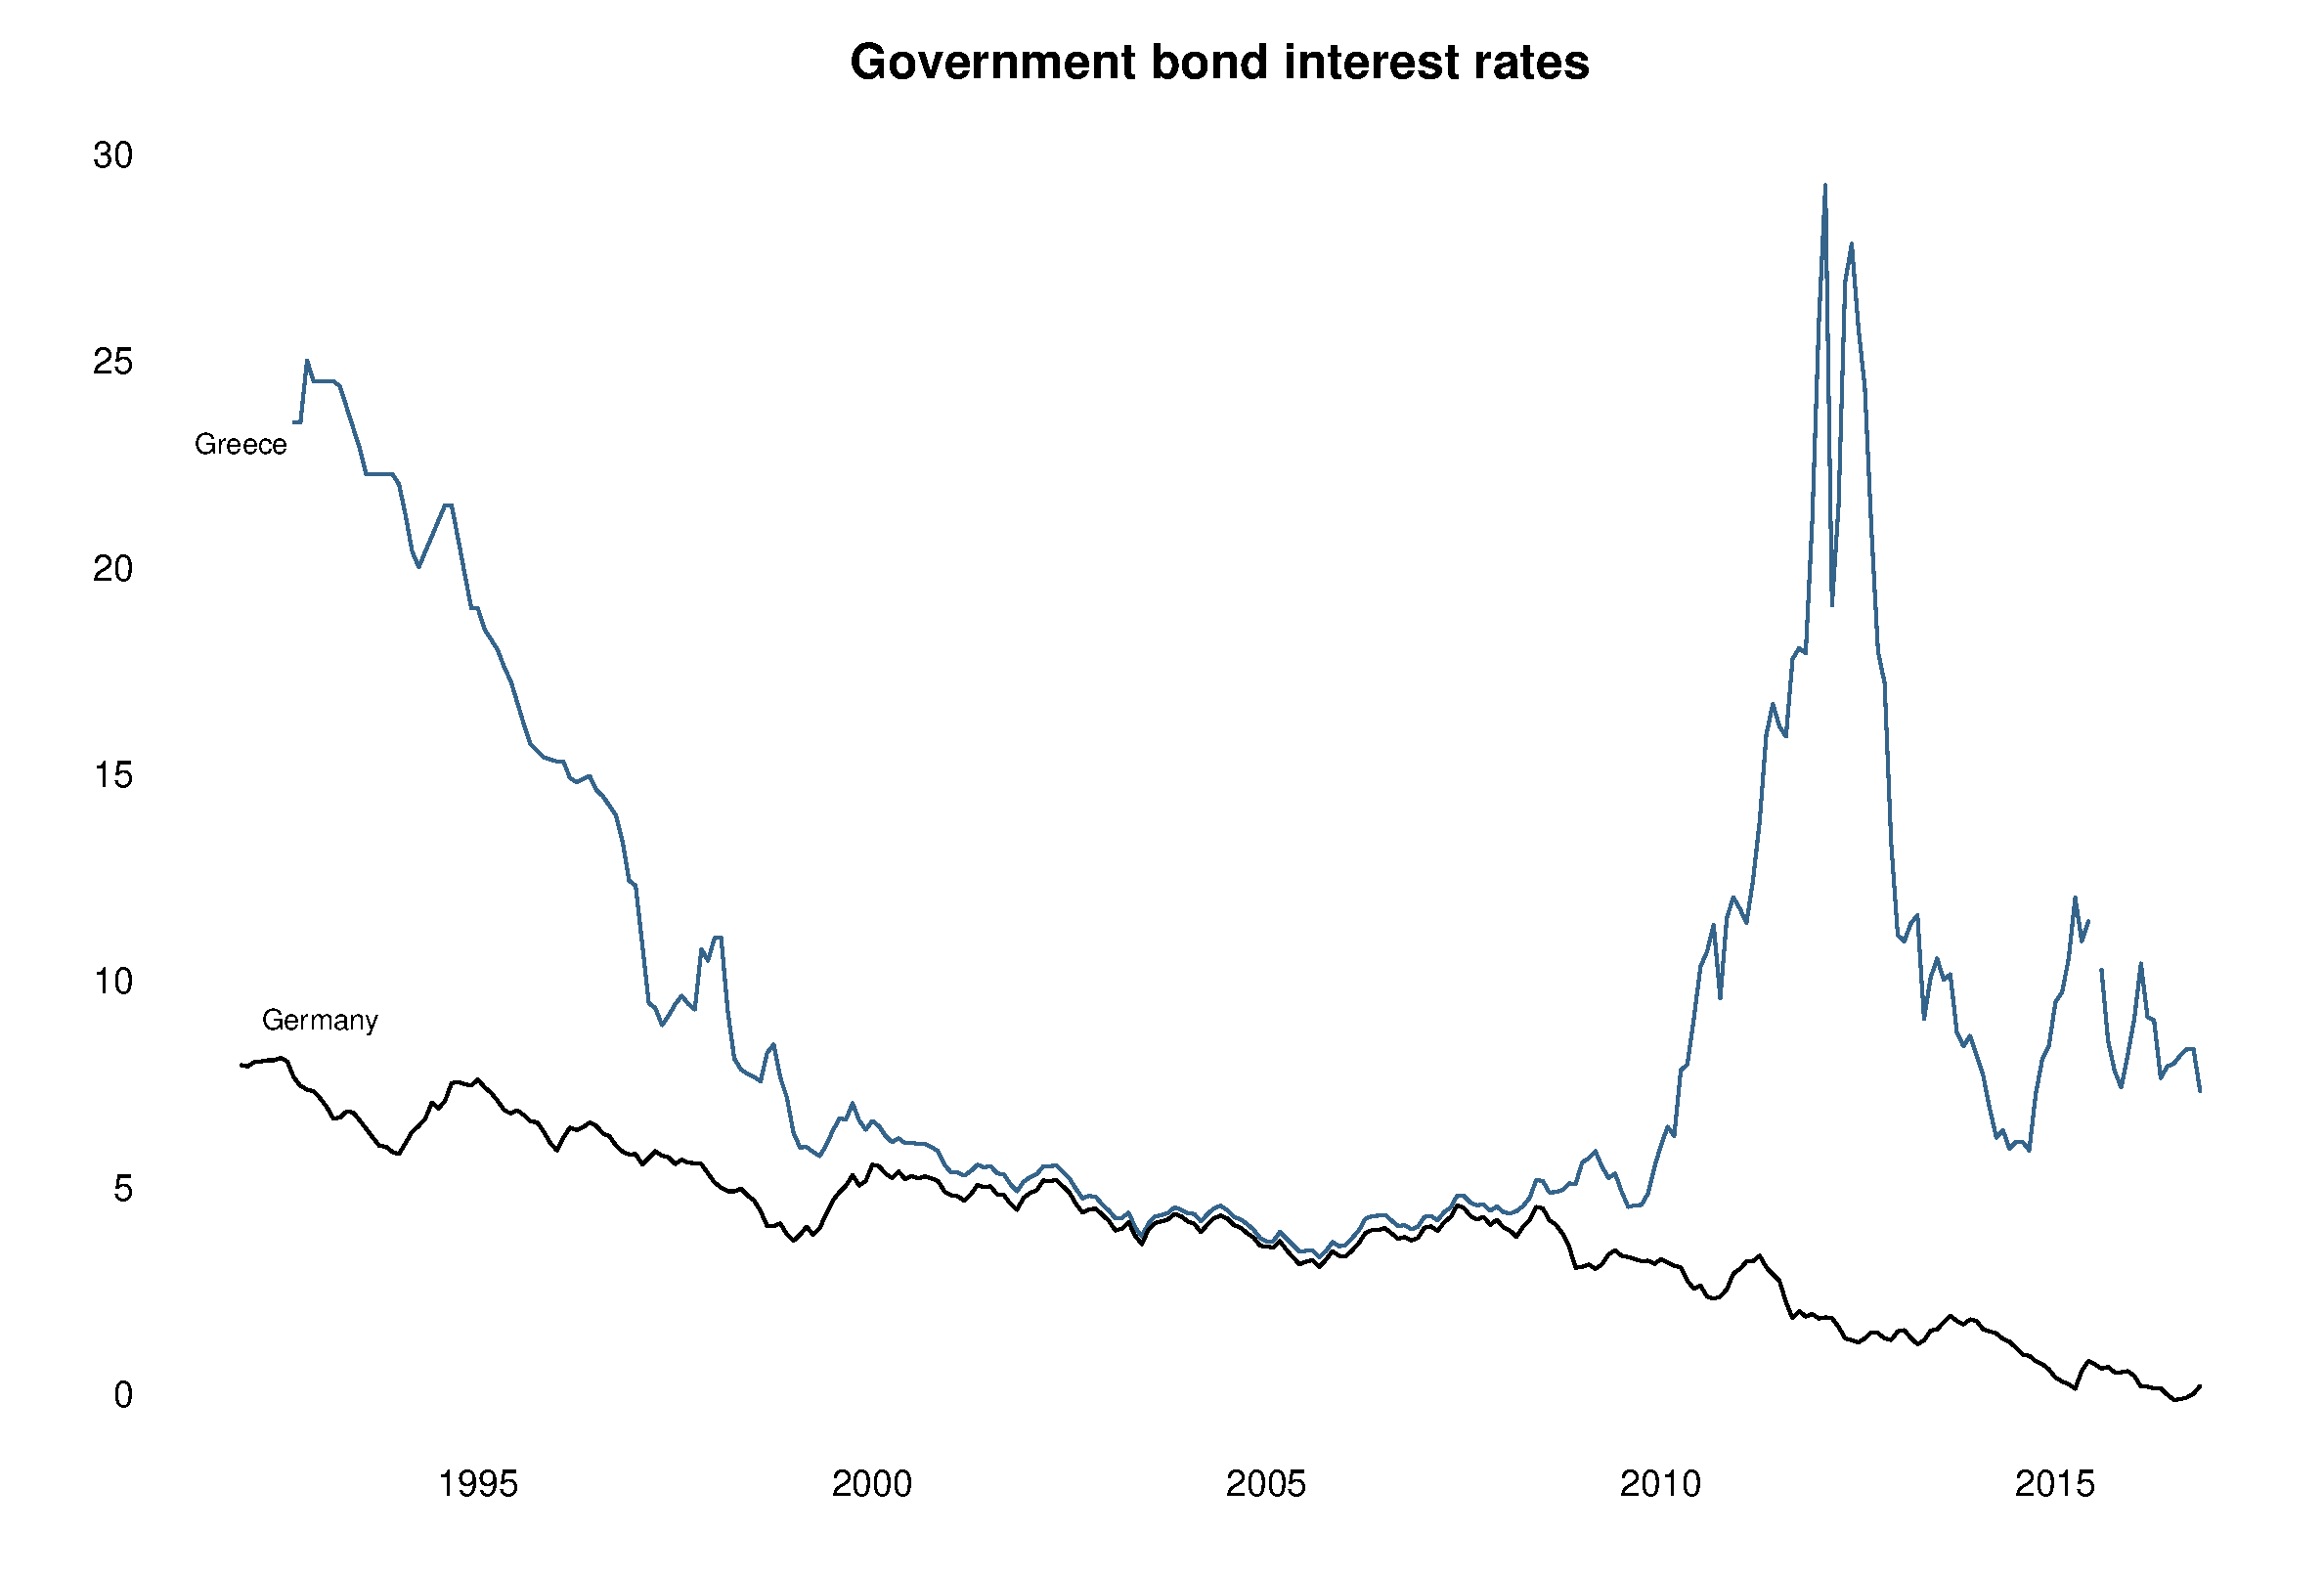
\includegraphics[scale=.3]{government_bonds.eps}
  \end{figure}
\end{frame}
%--------------------------------------

%--------------------------------------
\begin{frame}
  \textbf{Interest rate parity condition and risk}\\
  Greek Drachma was a weak currency vis-a-vis Deutschmark
  \begin{itemize}
    \item Perennially depreciating
    \item Reflected by higher interest rates
  \end{itemize}
  \medskip
  2001 Greece joined eurozone: fixing Drachme-Deutschmark exchange rate
  \begin{itemize}
    \item IRP conditions predict convergence of interest rates
  \end{itemize}
  \medskip  
  Divergence post-2009
  \begin{enumerate}
    \item Market expectation of Grexit
    \item \begin{align*} i^{GRC}_t = i^{GER}_t + \Pi_t    \end{align*}
 \end{enumerate}
\end{frame}
%--------------------------------------

%--------------------------------------
\begin{frame}
  Parity condition cannot be directly observed
  \begin{itemize}
    \item $E^e_{t+1}$ cannot be measured
    \item On whom does $E^e_{t+1}$ depend? 
  \end{itemize}  
 Interest rate parity condition shows \textbf{market sentiment}, revealing market expectations
  \begin{align}
      i_t &= i^*_t +  \frac{E^e_{t+1}}{E_t}\\ \nonumber
      i_t - i^*_t  &= \frac{E^e_{t+1}}{E_t}
  \end{align}
  i.e. expected exchange rate depreciation equals Domestic interest rate minus Foreign interest rate  
\end{frame}
%--------------------------------------

%--------------------------------------
\begin{frame}
  Given 
  \begin{align}
    i_t = i^*_t +  \frac{E^e_{t+1}}{E_t}
  \end{align}
   a country can 
  \begin{enumerate}
    \item Adjust $i$ to influence capital movement ($E_t$ varies)
    \item Adjust $E_t$ and set $i$ (no capital movement)
    \item Have capital movement and set $E_t$ (cannot set $i$)
  \end{enumerate}
\end{frame}
%--------------------------------------

%--------------------------------------
\begin{frame}
  \textbf{Impossible trinity principle}
  \begin{enumerate}
    \item Monetary autonomy
    \item Exchange-rate management
    \item Free capital mobility    
  \end{enumerate}
  \medskip
  Picking only two of of three is possible.
\end{frame}
%--------------------------------------

%--------------------------------------
\begin{frame}
  \begin{figure}
    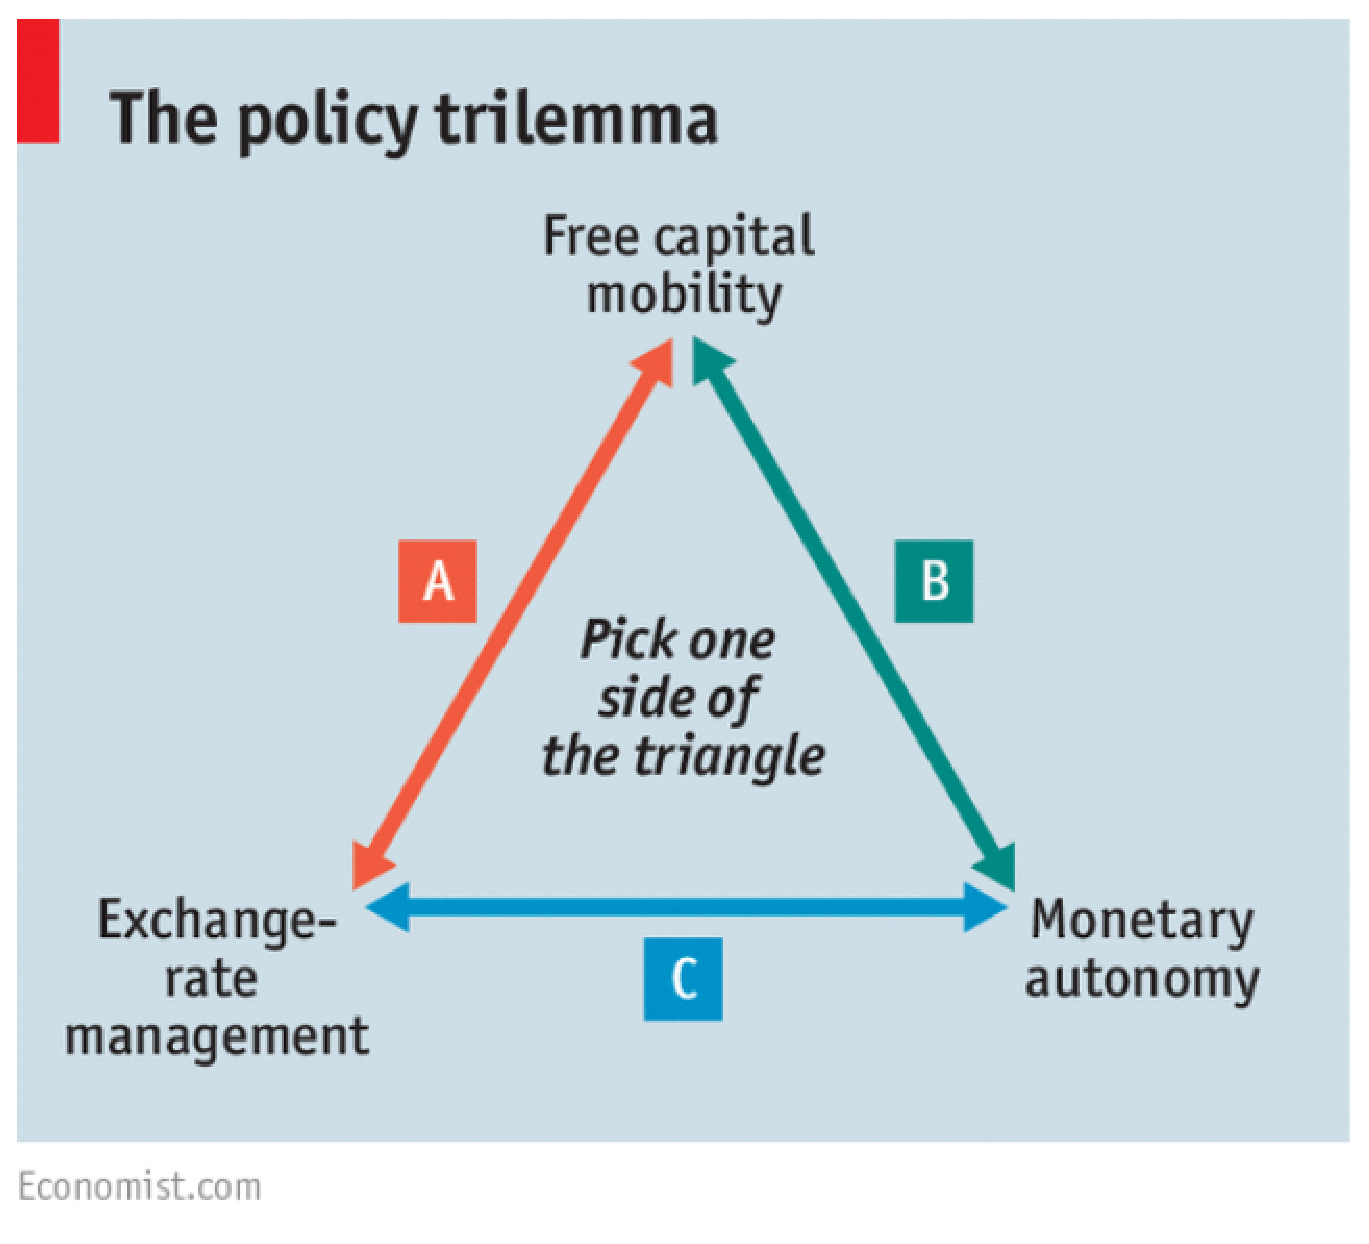
\includegraphics[scale=.4]{impossible_trinity.eps}
  \end{figure}
\end{frame}
%--------------------------------------



%--------------------------------------
\begin{frame}
  \begin{enumerate}
    \item Full capital mobility and autonomous monetary policy, flexible exchange rate
    \begin{itemize}
      \item Eurozone
      \item Volatile exchange rates could harm competitiveness
    \end{itemize}
    \medskip
    \item Full capital mobility and fixed exchange rate
    \begin{itemize}
      \item Bretton Woods system (1944-1973), Denmark
      \item Risk of current account deficits
    \end{itemize}
    \medskip
    \item Fixed exchange rate and monetary policy autonomy, with capital controls
    \begin{itemize}
      \item Brazil, China
      \item Need to enforce restrictions
    \end{itemize}
  \end{enumerate}
\end{frame}
%--------------------------------------

%--------------------------------------
\begin{frame}
  \begin{figure}
    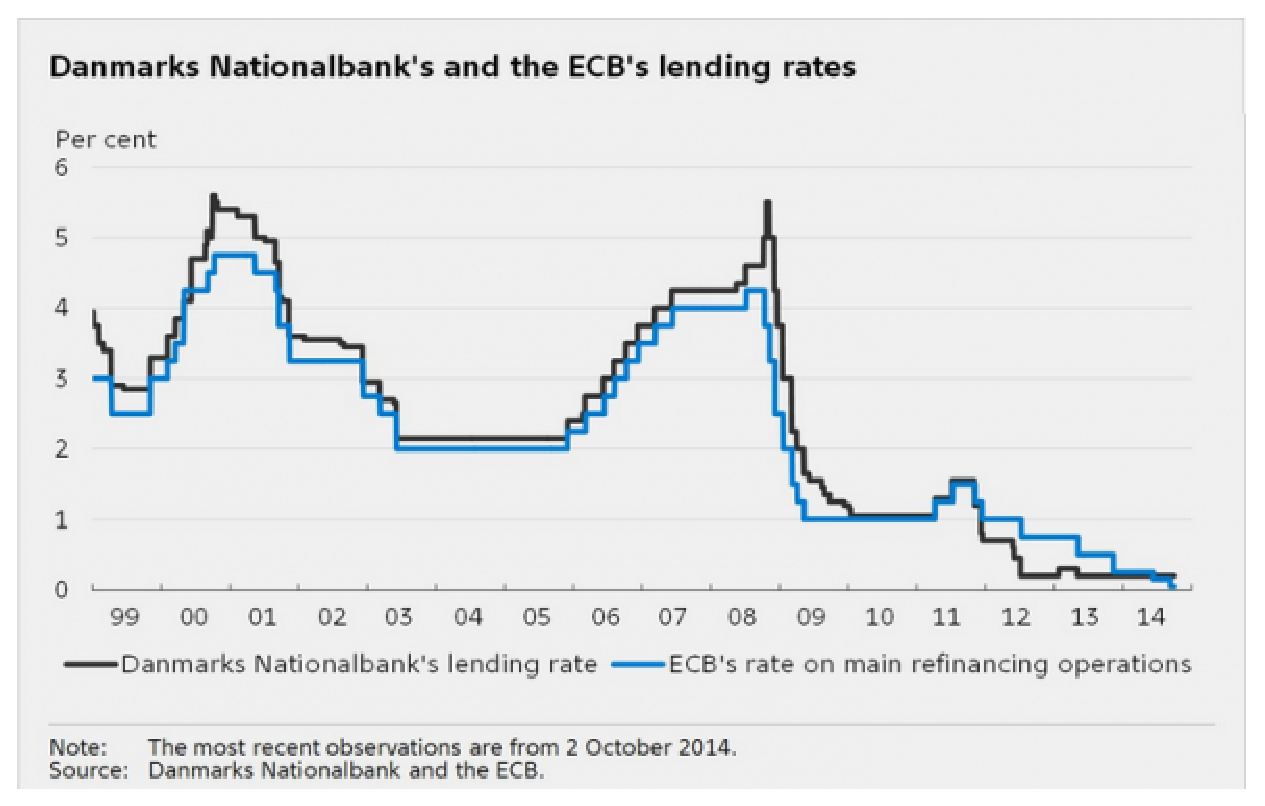
\includegraphics[scale=.5]{denmark.eps}
  \end{figure}
\end{frame}
%--------------------------------------

%--------------------------------------
\begin{frame}
  \textbf{Interest rate} set by central bank will affect price levels
  \begin{itemize}
    \item Recall, lower $i$ will increase spending
  \end{itemize}
  \medskip
  However, monetary policy loses influences after about 3 years
  \begin{itemize}
    \item Stronger demand leads to higher prices: erodes purchasing power
    \item Purchasing power inversely related to price level
  \end{itemize}
  \medskip
  \textbf{Monetary neutrality}
  \begin{quote}
      In the long run, monetary policy loses its effectiveness because the price level increases in the same proportion as the money stock
  \end{quote}  
\end{frame}
%--------------------------------------

%--------------------------------------
\begin{frame} 
  Can define  \textbf{real exchange rate} as 
  \begin{align}
    \frac{Ep}{p^*}
  \end{align}
  $p$, price for domestic good\\
  $p^*$, price for foreign good
  \begin{itemize}
    \item Relative price of domestic goods expressed in foreign goods
    \item Prices matter for competitiveness just as $E$
  \end{itemize}
  \medskip
  Rate appreciates when
  \begin{itemize}
    \item Nominal exchange rate $E$ appreciates
    \item $\frac{p}{p^*}$ increases, i.e. $p$ rises faster than $p^*$
  \end{itemize}
\end{frame}
%--------------------------------------

%--------------------------------------
\begin{frame}
  \textbf{Purchasing power parity (PPP) principle}
  \begin{align}
    \frac{E_t}{E_{t-1}} = \pi^* - \pi
  \end{align}
  $\pi$ is inflation rate.
  \begin{itemize}
    \item Rate of change of the nominal exchange rate is equal to the difference between inflation rates in two countries    
  \end{itemize}
  \medskip
  Currency should appreciate when
  \begin{align}
    \pi<\pi^*
  \end{align}
  \medskip
  Principle only holds in the long run (i.e. many many years)
\end{frame}
%--------------------------------------

%--------------------------------------
\begin{frame}
  Can also write PPP principle as
  \begin{align}
    E=\frac{p}{p^*}
  \end{align}
  \medskip
  i.e. the exchange rate reflects the relative price levels.\\
  PPP is based on the \textbf{Law of One Price}
  \begin{itemize}
     \item Does not hold in short-run
     \item Goods are not instantly tradeable (some are non-tradeable)
  \end{itemize} 
\end{frame}
%--------------------------------------

%--------------------------------------
\begin{frame}
  \begin{figure}
    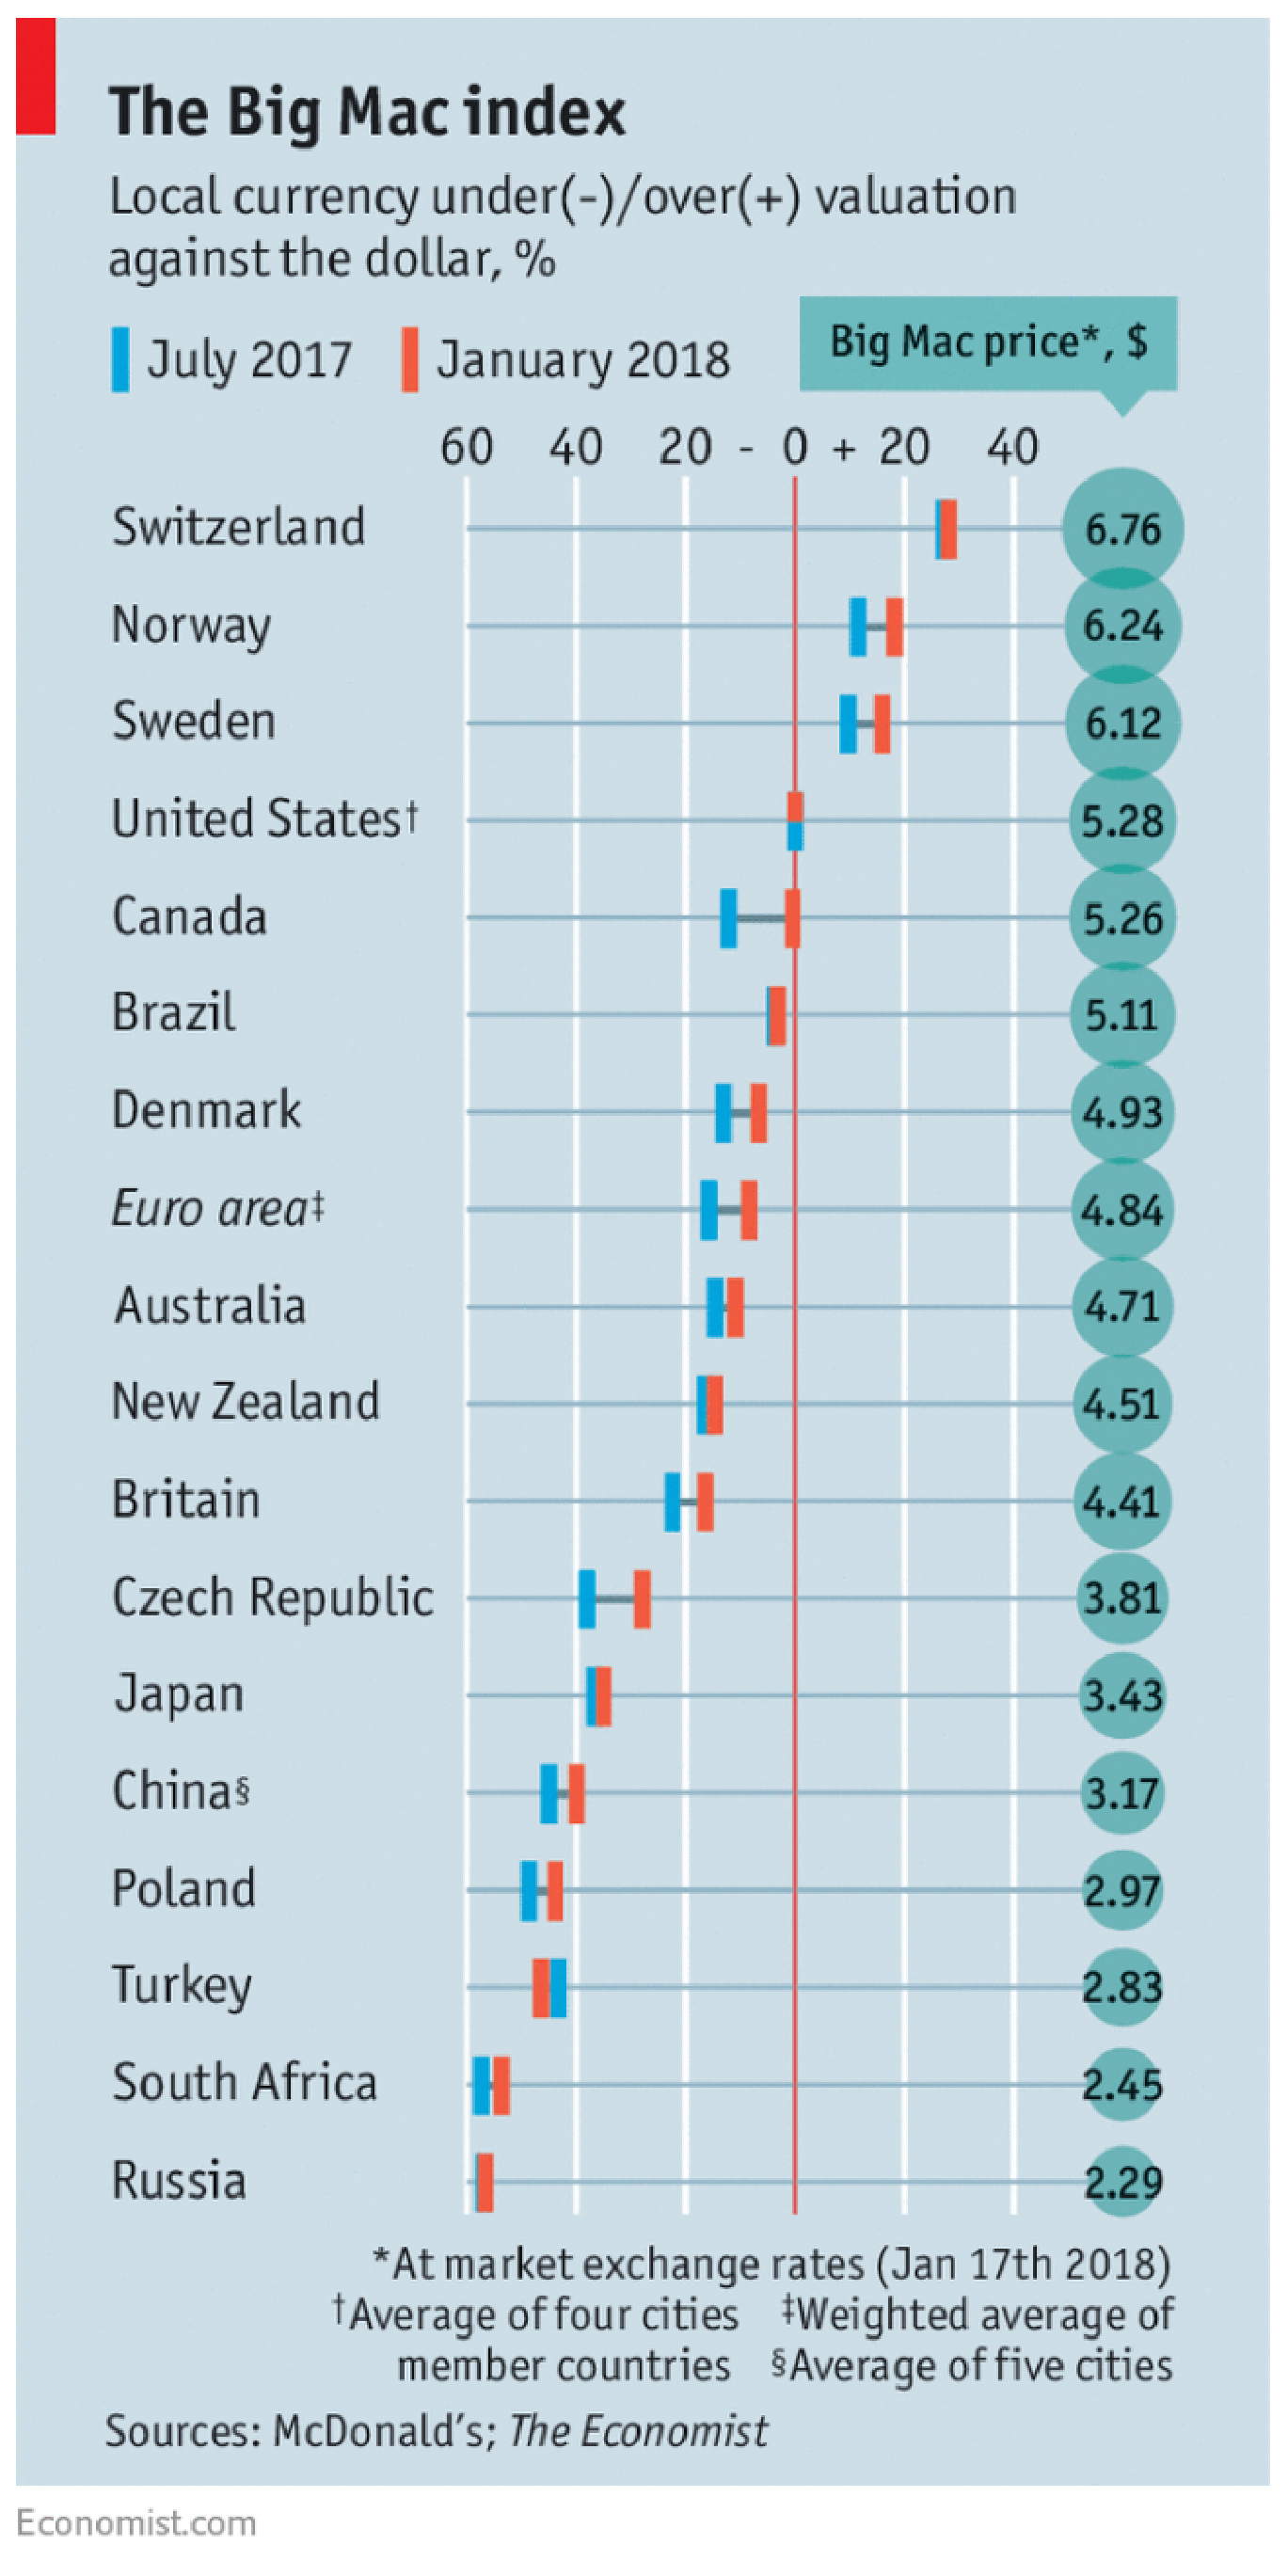
\includegraphics[scale=.2]{big_mac_index.eps}
  \end{figure}
\end{frame}
%--------------------------------------

%--------------------------------------
\begin{frame}
  \textbf{Equilibrium real exchange rate}\\
  PPP implies that $\frac{Ep}{p^*}$ is constant.\\
  Rate of change of real exchange rate can be given by
  \begin{align}
    \frac{\Delta \frac{Ep}{p^*}}{\frac{Ep}{p^*}}=  \frac{\Delta E}{E} + \frac{\Delta p}{p} - \frac{\Delta p^*}{p}
  \end{align}
  If follows that
  \begin{align}
    \frac{\Delta \frac{Ep}{p^*}}{\frac{Ep}{p^*}}=0
  \end{align}
  when
  \begin{align}
    \frac{\Delta E}{E} = \frac{\Delta p^*}{p^*} - \frac{\Delta p}{p}
  \end{align}
\end{frame}
%--------------------------------------


%--------------------------------------
\begin{frame}   
  Consider appreciation of real exchange rate
  \begin{itemize}
    \item e.g. introduction of Euro
  \end{itemize}
  \medskip
  Country becomes less competitive (increase in price level)
  \begin{itemize}
    \item Exports decline: domestic goods are more expensive on foreign markets
    \item Imports increase: foreign goods cheaper at home
  \end{itemize}
  \begin{align}
    X<M
  \end{align}
  \medskip
  Deficit needs to be financed through borrowing abroad  
\end{frame}
%--------------------------------------

%--------------------------------------
\begin{frame}
  For real exchange rate to return to equilibrium one of two things need to happen
  \medskip
  \begin{enumerate}
    \item Depreciation of nominal exchange rate
    \begin{itemize}
      \item Need to be able to manage exchange rate
    \end{itemize}
    \medskip
    \item Prices must move to re-establish competitiveness
    \begin{itemize}
      \item Will have effect on wages
    \end{itemize}
  \end{enumerate}
\end{frame}
%--------------------------------------

%--------------------------------------
\begin{frame}
  \textbf{Balassa-Samuelson effect}
  \begin{quote}
    Equilibrium real exchange rates of countries that enjoy lasting fast growth - because they are catching up from a lower level of development - follow an appreciating trend
  \end{quote}
  \medskip
  By-product of catch-up process 
  \begin{itemize}
    \item Relatively underdeveloped countries gradually close the technology gap between themselves and advanced countries.
  \end{itemize}  
\end{frame}
%--------------------------------------

%--------------------------------------
\begin{frame}
  \begin{figure}
    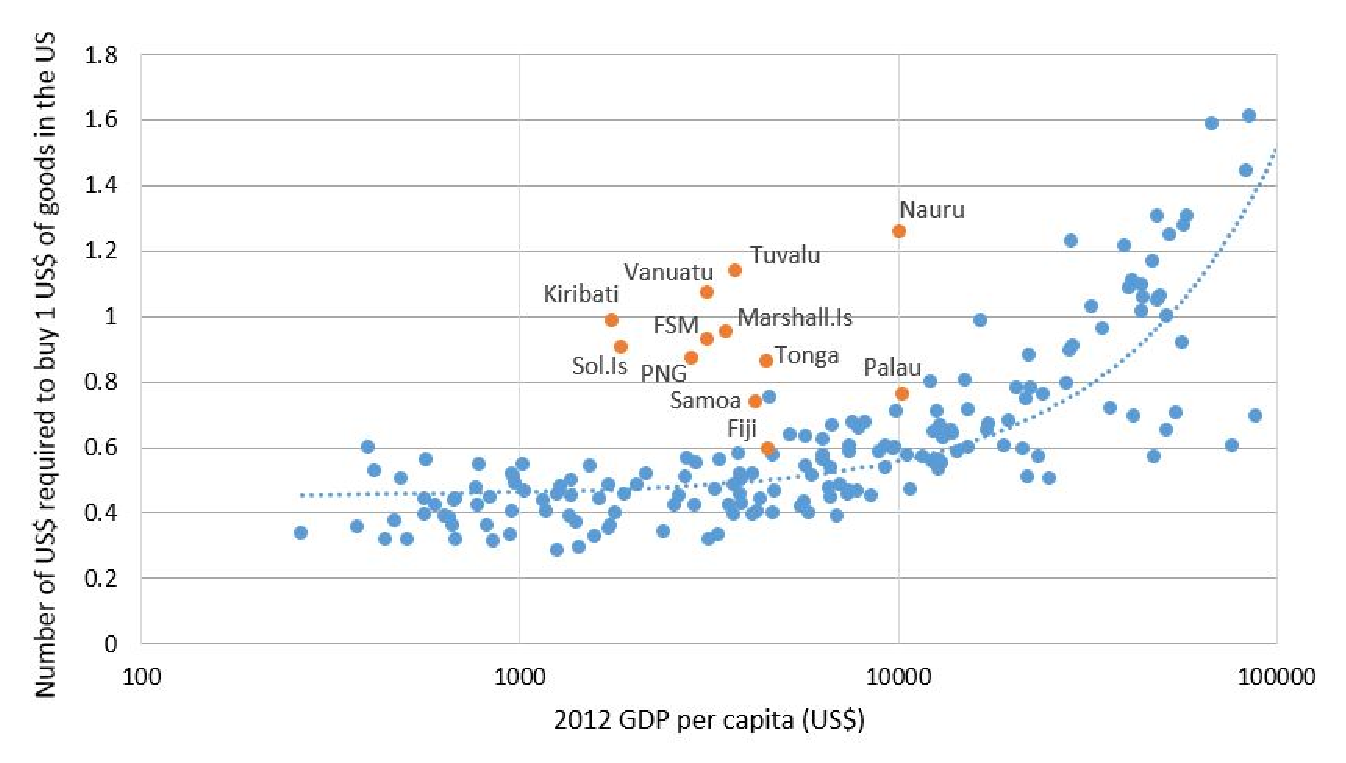
\includegraphics[scale=.5]{expensive_pacific.eps}
  \end{figure}
  Source: devpolicy.org
\end{frame}
%--------------------------------------

%--------------------------------------
\begin{frame}
  The Balassa-Samuelson effect happens when
 \begin{itemize}
    \item $Ep/p^*$ is steadily increasing as domestic prices rise relative to foreign prices evaluated in domestic currency $p^*/E$
    \item Or when domestic prices evaluated in foreign currency $Ep$ rise relative to foreign prices $p^*$
  \end{itemize}
  \medskip
  Real appreciation can happen due to
  \begin{enumerate}
    \item Higher inflation at home: $p / p^*$ increasing
    \item Continuous nominal appreciation: rising trend in $E$
  \end{enumerate}
  or combination of these two.
\end{frame}
%--------------------------------------

%--------------------------------------
\end{document}
